\documentclass[10pt]{article}
\usepackage[portuguese]{babel}
\usepackage[a4paper, top = 0.8in, bottom = 0.9in, left =0.6in, right = 0.6in]{geometry}
\usepackage{inputenc}
\usepackage{fancyhdr}
\usepackage{multirow}
\usepackage{graphicx}
\usepackage{times}
\usepackage{subcaption}
\usepackage{booktabs}
\usepackage{microtype}
\usepackage{wrapfig}
\usepackage{circuitikz}
\usepackage{titlesec}
\usepackage{wrapfig}
\usepackage{listings}
\usepackage{tikz}

\usepackage{caption}
\usepackage{ragged2e}
\usepackage{adjustbox}
\usepackage{float}
\usepackage{amsmath, mathtools, amssymb}
\usepackage{parskip}
\usepackage{array, makecell}
\usepackage{booktabs}
\titleformat{\section}
{\normalfont\large\bfseries}{\thesection)}{1em}{}
\titleformat{\subsection}
{\normalfont\normalsize\bfseries}{\thesubsection)}{1em}{}
\titleformat{\subsubsection}
{\normalfont\normalsize\bfseries}{\thesubsubsection)}{1em}{}


%\pretitle{\begin{center}\Huge\bfseries}

\pagestyle{fancy}
\fancyhead{}
\centering\chead{
\includegraphics[width=15cm]{imagens/unb_fga_logo_extenso.jpg}}
\lfoot{Prática de Circuitos 1 - 2020/1}
\rfoot{\textbf{Prof. Dr. Marcus V. Chaffim Costa}} %nome do rodape
\renewcommand{\footrulewidth}{1pt}

\setlength{\parskip}{0.1cm}
\author{Monitoria - 2019/2}
\title{Tutorial 0}


%arrumação das tabelas

\setlength{\tabcolsep}{0.5em} % for the horizontal padding
{\renewcommand{\arraystretch}{1.2}}% for the vertical padding
\captionsetup[table]{name= \bfseries Tabela}
\captionsetup[figure]{name= \bfseries Figura}
\numberwithin{table}{section}
\numberwithin{figure}{section}
\usepackage{array}
\newcolumntype{C}[1]{>{\centering\arraybackslash}m{#1}}

\aboverulesep=0cm
\belowrulesep=0cm

%configuracoes dos codigos em matlab

\usepackage{color} %red, green, blue, yellow, cyan, magenta, black, white
\definecolor{mygreen}{RGB}{28,172,0} % color values Red, Green, Blue
\definecolor{mylilas}{RGB}{170,55,241}

\lstset{language=Matlab,%
    %basicstyle=\color{red},
    breaklines=true,%
    morekeywords={matlab2tikz},
    keywordstyle=\color{blue},%
    morekeywords=[2]{1}, keywordstyle=[2]{\color{black}},
    identifierstyle=\color{black},%
    stringstyle=\color{mylilas},
    commentstyle=\color{mygreen},%
    showstringspaces=false,%without this there will be a symbol in the places where there is a space
    numbers=left,%
    numberstyle={\tiny \color{black}},% size of the numbers
    numbersep=9pt, % this defines how far the numbers are from the text
    emph=[1]{for,end,break},emphstyle=[1]\color{red}, %some words to emphasise
    %emph=[2]{word1,word2}, emphstyle=[2]{style},    
}

\allowdisplaybreaks


%==============macros para uso nos documentos===================%

\newcommand{\ohm}{\Omega}


\newcommand{\figuras}[4]{
    \begin{figure}[H]
        \centering
        \includegraphics[width={#1}\textwidth]{#2}
        \caption{#3}
        \label{fig:#4}
    \end{figure}
}

\newcommand{\figura}[2]{
    \begin{figure}[H]
        \centering
        \includegraphics[width=#1\textwidth]{#2}
    \end{figure}
}

\newcommand{\subfiguras}[5]{
    \centering
    \begin{subfigure}[H]{#1\textwidth}
        \centering
        \includegraphics[width={#2}\textwidth]{{#3}}
        \caption{{#4}}
        \label{fig:{#5}}
    \end{subfigure}
}

\newcommand{\circuito}[3]{
    \begin{figure}[H]
        \centering
        \begin{circuitikz}[line width=.5pt]
            #1
        \end{circuitikz}
        \caption{{#2}}
        \label{circ:{#3}}    
    \end{figure}
}

\newcommand{\calc}[1]{
    \begin{gather*}
        #1
    \end{gather*}
}





%=====================================================%

\usetikzlibrary{automata}

\begin{document}

\begin{center}
\vspace*{.03cm}
\Large\textbf{Experimento 01:}\\ %titulo
\Large{Instrumentos de Bancada e Geração de Sinais AC}
\end{center}
\justify

\section{Objetivos}

Nesta experiência prosseguimos com a investigação dos demais instrumentos de bancada do laboratório a fim de compreender
seu funcionamento. Então, produziremos sinais AC, a partir dos quais aferiremos parâmetros, com o intuito de aprender a operar
adequadamente os equipamentos e desenvolver conceitos de amplitude, frequência, valor médio e valor eficaz de um sinal.

\section{Objetivos}
Nesta experiência investigaremos alguns dos instrumentos de bancada do laboratório a fim de compreender como
funcionam. Em seguida produziremos sinais DC e realizaremos medições de tensão,corrente e resistência. O intuito é desenvolver habilidades na manipulação dos equipamentos.

\section{Estudo pré-laboratorial}

\subsection{Instrumentos de Bancada}

\subsubsection{Fonte de alimentação}

\begin{itemize}
    \item \textbf{O que é faixa de tensão de saída do equipamento?}
        
        É a faixa de tensões em que o aparelho fornece em sua saída. Ela pode ser limitada nominalmente pelo usuário através de um potenciômetro (em algumas literaturas, \textit{knob}). A faixa de tensões vária em função do modo de operação escolhido entre os canais de saída da fonte.

    \item \textbf{O que é faixa de corrente de saída do equipamento?}

        É a faixa de corrente que o aparelho fornece em sua saída. É análogo à faixa de tensões, mas conta, vale ressaltar, com o ajuste de corrente limite. A faixa de corrente também vária em função do modo de operação configurada na fonte.
    \item \textbf{O que é corrente limite?}

        É a corrente máxima configurada pelo usuário a partir da qual a proteção contra sobrecorrente atua. A quantidade de corrente opera a partir da resistência oferecida pelo circuito, ou seja, se há algum componente que esteja danificado, há probabilidades que haja o sobreaquecimento e, com isso, até a combustão do componente.
\end{itemize}

\subsubsection{Modos de Operação de Fontes de Alimentação}

Atualmente há, majoritariamente, dois tipos de fonte no laboratório: MPL-1303 e MPL-3305, ambas da Minipa e, portanto, compartilham do mesmo manual. A principal diferença reside entre a quantidade de canais de saída existentes: a MPL-1303 possui apenas um canal de saída, enquanto a MPL-3305 possui dois canais de saída. Implica-se, então, que a MPL-1303 possui apenas o modo de operação simples.

Para todas os modos de operação, devemos configurar as teclas de Seleção do Modo de Conexão (também conhecidas como Teclas de Tracking). Elas mudam a conexão entre as fontes de acordo com as associações desejadas. As configurações de Tracking dos modos Independente, Série ou paralelo para a fonte MPL-3305 estão elencados abaixo:

\figuras{.5}{imagens/instr_banc/tracking}{Configurações de Conexão}{tracking}

\begin{itemize}
     
    \item \textbf{Fixa}

        A fonte MPL-3305 conta com três saídas, sendo duas variáveis e uma fixa de 5V.
        
        \newpage

    \item \textbf{Simples}

        É o modo onde os canais de saída operam independentemente. A corrente máxima é de 5A.

        \figuras{.5}{imagens/instr_banc/op_simples}{Modo de Operação Simples.}{op_simples}
    \item \textbf{Paralelo}

        Nessa condição, os canais operam paralelamente e, consequentemente, as corrente se somam. A corrente máxima é, portanto, 10A.

        \figuras{.4}{imagens/instr_banc/op_paralelo}{Modo de Operação Paralela.}{op_paralelo}

    \item \textbf{Série}

        Nessa condição, os canais operam em serialmente e, consequentemente, as tensões se somam. A tensão máxima é 64V.

        \figuras{.4}{imagens/instr_banc/op_serie}{Modo de Operação Série.}{op_serie}
    \item \textbf{Simétrica}
    
        Nesta condição, pode-se conseguir um terra comum para ambos os canais variáveis, com saída positiva e negativa de, no máximo, +32V e -32V, respectivamente. 
    
        \figuras{.4}{imagens/instr_banc/op_simetric}{Modo de Operação Simétrica.}{op_simetrica}
\end{itemize}

O ajuste de corrente limite é ilustrado na figura abaixo:

\figuras{.4}{imagens/instr_banc/corr_lim}{Configuração da Corrente Limite na fonte MPL-3305}{}

Observe que, propositalmente, não houve um detalhamento das peculiaridades de cada um dos modos de operação. Através dos manuais dos equipamentos, procure compreender o modo de funcionamento das fontes de alimentação. Como guia, responda as seguintes perguntas:

a) Fonte de alimentação modelo MPL-1303 Minipa:

\begin{itemize}
    \item Qual a faixa de tensão de saída desse equipamento?
    \item Qual a faixa de corrente de saída desse equipamento?
    \item Como definir um valor máximo de corrente de saída para a fonte (corrente limite)?
\end{itemize}

\vspace{.5em}

b) Fonte de alimentação modelo MPL-3305 Minipa:

\begin{itemize}
    \item Qual a faixa de tensão de saída para esse equipamento?
    \item Qual a faixa de corrente de saída para esse equipamento?
    \item Quais os limites de tensão e corrente obtidos em cada um dos modos de operação?
\end{itemize}

\subsubsection{Multímetro}

\begin{itemize}
    \item \textbf{Medição de Tensão com Multímetro:}Posicione a chave rotativa para medição de voltagem contínua e conecte as pontas de prova em paralelo no circuito em teste.
    
    \figuras{.2}{imagens/instr_banc/mult_tens}{Medição de tensão com o multímetro.}{tens_mult}

    \item \textbf{Medição de corrente com o Multímetro:} Posicione a chave rotativa na maior escala possível de corrente e ajuste para uma visualização adequada. Conecte as pontas de prova em série no local a ser medido.
    
    \figuras{.35}{imagens/instr_banc/corr_mult}{Medição de corrente com o multímetro.}{corr_mult}
    
    \item \textbf{Medição de Resistência com o multímetro:} Posicione a chave rotativa em "$\ohm$". Conecte as pontas de prova sobre o objeto a ser medido.
    
    \figuras{.2}{imagens/instr_banc/res_mult}{Medição de Resistência com o multímetro.}{res_mult}

    \item \textbf{Integridade de Trilhas:} Posicione a chave rotativa para medição de continuidade. O aparelho sonoriza um \textit{beep} quando a resistência de um circuito for menor que $10\ohm$.
    
    \figuras{.2}{imagens/instr_banc/int_trilh}{Teste de integridade de trilhas com o multímetro.}{int_trilh}
\end{itemize}

Assim como as fontes de tensão, há dois modelos de multímetro disponíveis no laboratório atualmente: ET-1110 da Minipa e o TOOZ DT830 Series. Estude a manipulação e as características nos manuais do aparelho.




\section{Simulações}
Para senóides com $f =100 Hz$ e resistores (em Ohms), respectivamente, $R_1 = 100\Omega$, $R_2 = 560\Omega$, $R_3 = 220\Omega$ e $R_4 = 330\Omega$, simule os circuitos A, B e C para todas as combinações de V1, V2 e V3 apresentadas na \textbf{Tabela 1} da \textbf{Folha de Dados}.

\subsection{Circuito A}


\begin{itemize}
    \item Inicialmente, abra o QUCS, vá em \textit{Main Dock} e crie uma nova pasta de projeto. 
    
    \item Na aba Componentes (\textit{Components}), vá em componentes não lineares (\textit{non linar components}) e clique em um Amplificador Operacional (\textit{OpAmp}). Em componentes agrupados (\textit{lumped components}) e clique em dois resistores. Vá em Fontes (\textit{sources}) e coloque uma fonte de tensão AC (\textit{AC voltage Source}).
\end{itemize}

\begin{figure}[H]
    \begin{subfigure}{.4\textwidth}
        \centering
        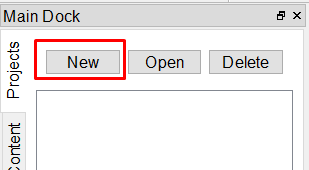
\includegraphics[width=.7\textwidth]{imagens/CircuitoA/new.png}
        \caption{Criação de um novo Projeto}
        \label{fig:new_proj}
    \end{subfigure}    
    \begin{subfigure}{.4\textwidth}
        \centering
        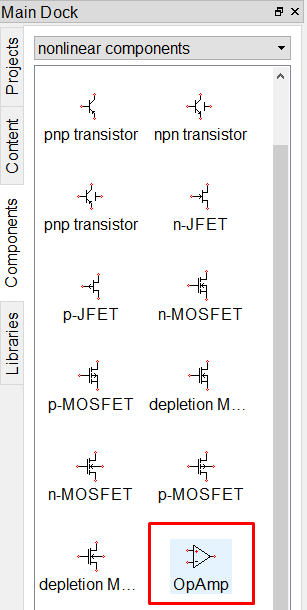
\includegraphics[width=.7\textwidth, trim={ 0 0 0 9cm}, clip]{imagens/CircuitoA/OpAmp.png}
        \caption{Seleção do Amp Op.}
        \label{fig:sel_ampop}
    \end{subfigure}
    
    \begin{subfigure}{.4\textwidth}
        \centering
        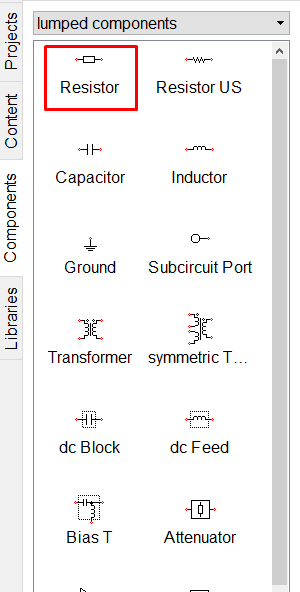
\includegraphics[width=.7\textwidth,  trim={0 7cm 0 0}, clip]{imagens/CircuitoA/resistor.png}
        \caption{Seleção do Resistor.}
        \label{fig:sel_res}
    \end{subfigure}
    \begin{subfigure}{.4\textwidth}
        \centering
        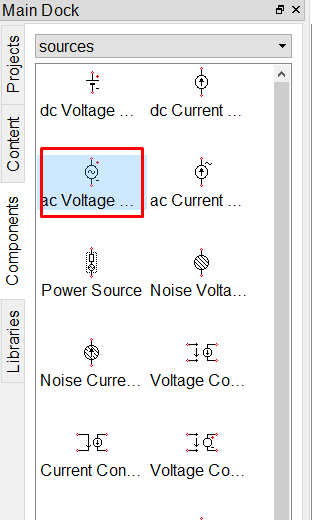
\includegraphics[width=.7\textwidth,  trim={0 7cm 0 0}, clip]{imagens/CircuitoA/fonto_ac.png}
        \caption{Seleção da fonte AC}
        \label{fig:new_proj}
    \end{subfigure}

    \caption{Abertura do projeto e seleção dos componentes }
\end{figure}

\begin{itemize}
    \item Conecte os componentes como a figura \ref{fig:circ_a_q}. Não se esqueça da referência e ajustar os valores dos resistores.
    \item É importante salientar que para essa simulação, necessitaremos de uma simulação AC e outra DC. A simulação AC é necessária para a fonte de voltagem AC, enquanto a fonte DC tem sua utilidade na ligação DC do Amplificador Operacional, \textit{i.e.}, tem seu efeito na energização do $V_{dd}$ e $V_{ss}$ do Amp Op.
    \item  Configure a Simulação AC para observar o valor da saída para a frequência desejada. Salve e simule.
    \item Vá em \textit{Diagramas} e insira uma tabela. Coloque o valor da tensão $V_o.v$. O resultado final deve ser igual ao representado na Figura \ref{fig:circ_a_q}.
    
    \begin{figure}[H]
        \centering
        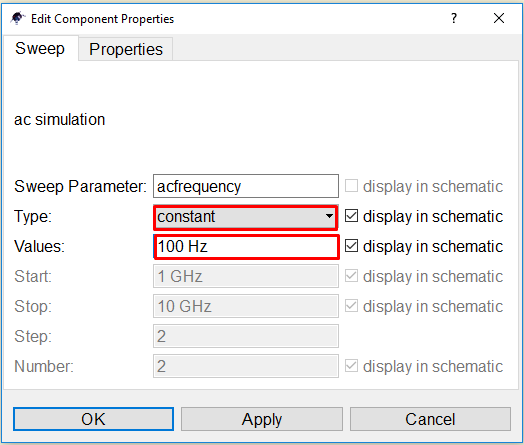
\includegraphics[width=.5\textwidth]{imagens/CircuitoA/simulacao.png}
        \caption{Parâmetros de Simulação AC.}
        \label{fig:my_label}
    \end{figure}
    
\end{itemize}


\begin{figure}[H]
    \centering
    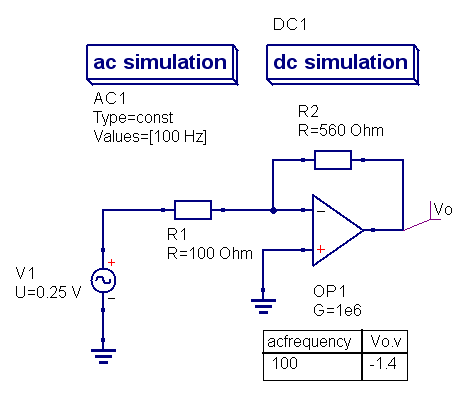
\includegraphics[width=.5\textwidth]{imagens/CircuitoA/circuito_a_sim.png}
    \caption{Arranjo do Circuito A no QUCS.}
    \label{fig:circ_a_q}
\end{figure}

\subsection{Circuito B}
    \begin{itemize}
        \item Vá em arquivo e clique em \textit{Salvar como} e mude o nome do arquivo para utilizar o esquemático já montado para o próximo circuito.
        \item Na aba \textit{Componentes}, vá em componentes agrupados e coloque mais dois resistores. Vá em Fontes e coloque mais duas fontes de tensão AC.
        \item Há duas formas de gerar os circuitos: gerar um por vez, cada qual com seu arquivo; gerar todos de uma só vez, num único arquivo (recomendado).
        \item Nesse tutorial, foi feito todas as variações da tabela 1 da folha de dados em um esquemáticos distintos, como ilustrado nas figuras \ref{fig:2_fon_des}, \ref{fig:1_fon_des} e \ref{fig:0_fon_des}.
    \end{itemize}

\begin{figure}[H]
   
    \begin{subfigure}{.4\textwidth}
        \centering
        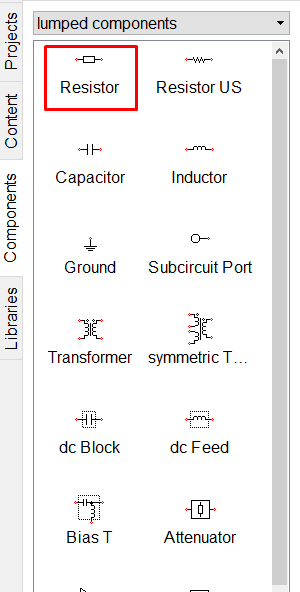
\includegraphics[width=.7\textwidth, trim={0 9cm 0 0}, clip]{imagens/CircuitoA/resistor.png}
        \caption{Seleção dos Resistores}
        \label{fig:sel_resis}
    \end{subfigure}
    \begin{subfigure}{.4\textwidth}
        \centering
        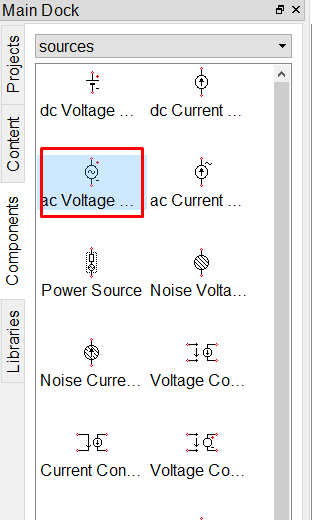
\includegraphics[width=.7\textwidth, trim={0 7cm 0 0}, clip]{imagens/CircuitoA/fonto_ac.png}
        \caption{Seleção fonte AC}
        \label{fig:sel_font_ac}
    \end{subfigure}    
    
 \begin{subfigure}{.45\textwidth}
        \centering
        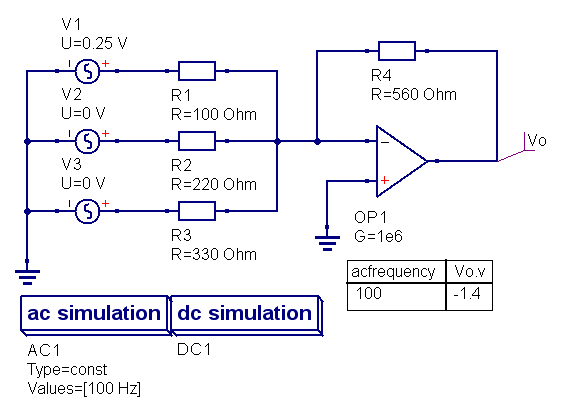
\includegraphics[width=\textwidth]{imagens/CircuitoB/-1_4.png}
        \caption{Uma fonte desativada}
        \label{fig:2_fon_des}
    \end{subfigure}    
    \begin{subfigure}{.45\textwidth}
        \centering
        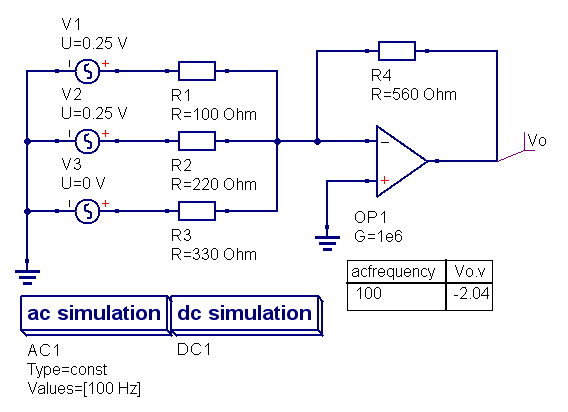
\includegraphics[width=\textwidth]{imagens/CircuitoB/-2_04.png}
        \caption{Apenas uma fonte desativada}
        \label{fig:1_fon_des}
    \end{subfigure}
    \centering
    \begin{subfigure}{.45\textwidth}
        \centering
        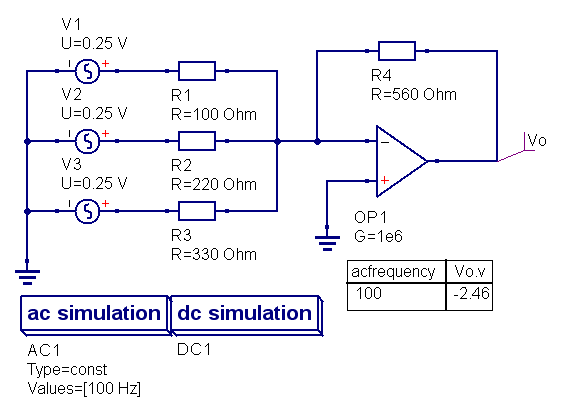
\includegraphics[width=\textwidth]{imagens/CircuitoB/-2_46.png}
        \caption{Todas as fontes Ativas}
        \label{fig:0_fon_des}
     \end{subfigure}
\end{figure}



\subsection{Circuito C}


    \begin{itemize}
        \item Vá em Arquivo e depois em Salvar como... e mude o nome do arquivo para utilizar o esquemático já montado para a o próximo circuito. Exclua a Fonte $V_3$ e conecte os componentes sem esquecer da referência do terra.
        \item Copie  e cole o circuito e modifique os valores das fontes para $V_1 = 0,5V_{pp}$ e $V_2=0V_{pp}$.
        \item Copie e cole em outro espaço, novamente, e modifique os valores das fontes para $V_1 = 0V_{pp}$ e $V_2=0,5V_{pp}$.
        \item Salve e simule.
        \item Vá em Diagramas e insira uma tabela. Coloque o valor das tensões.
        \item Nesse ponto do tutorial, foi colocado todos os circuitos em um único esquemático.
        \item O resultado obtido deve ser semelhante ao apresentado na figura \ref{fig:circuito_c_sim}.
    \end{itemize}

    \begin{figure}[H]
        \centering
        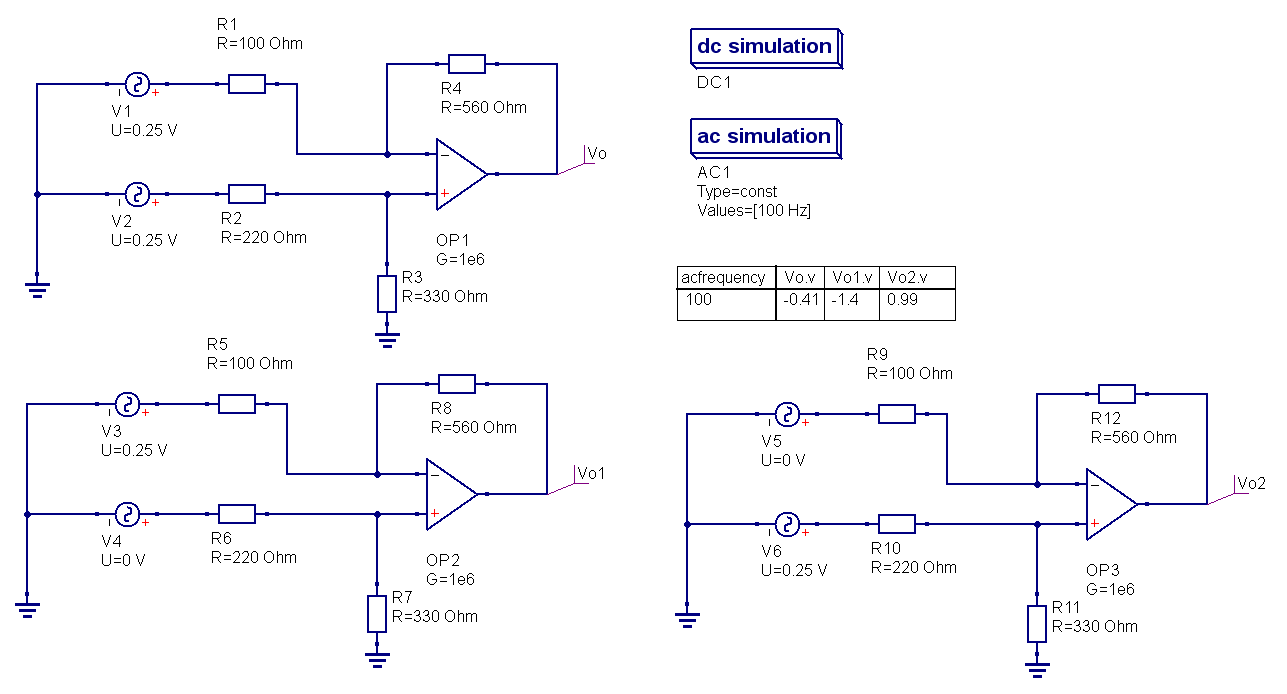
\includegraphics[width=\textwidth]{imagens/CircuitoC/sim_c.png}
        \caption{Esquemático do circuito montado}
        \label{fig:circuito_c_sim}
    \end{figure}
\newpage
\section{Experimento}

\subsection{Multímetro}

\noindent a) Meça com o multímetro o valor dos resistores disponíveis em cima da bancada. Confira o valor nominal indicado pelo código
de cores e calcule o erro percentual. Verifique se ele se encontra dentro da tolerância especificada pelo fabricante do resistor.

\subsection{Geração de tensões}

\noindent a) Use a fonte de alimentação e escolha o modo de operação mais apropriado para obter os seguintes sinais de tensão DC:

\begin{itemize}
    \item +10 V e -10 V c/ terra comum (máx 3 A);
    \item 40 V (máx 3 A);
    \item 5 V (máx 6 A);
    \item 5 V (máx 3 A);
    \item 10 V (máx 3 A);
\end{itemize}

Verifique os valores obtidos com o auxílio do multímetro e comente sobre o resultado.

\noindent b) Monte o circuito da Figura 11, utilizando o resistor $R = 100 \ohm$ e ajuste a fonte de alimentação em 3 V, 5 V e 10 V. Meça a tensão e a corrente sobre o resistor R em cada caso. Discuta os valores observados e compare-os com os obtidos nos cálculos teóricos da sessão 3.1, justificando os valores observados.

\subsection{Modo tensão/corrente constante}

\noindent a) Ajuste a fonte de alimentação para fornecer uma tensão de 10 V e corrente máxima de 30 mA.

b) Monte o circuito da Figura 12, com $R = 100 \ohm$ e substituindo o resistor R2 pelo potenciômetro ajustado para os seguintes valores:

\begin{itemize}
    \item $1 k\ohm$;
    \item $500 \ohm$;
    \item $200 \ohm$;
    \item $100 \ohm$;
    \item $50 \ohm$.
\end{itemize}


Em seguida, verifique com o multímetro os valores de tensão $V_f$ e corrente $i_f$ fornecidos pela fonte para diferentes valores de $R_2$.
Explique o que você observou e justifique o comportamento da fonte comparando com os cálculos teóricos de $V_f$ e $i_f$ realizados
nas simulações.

\end{document}